% Overview:
%   Main TeX file for the project.
%   Subfiles should reside in the sections/ directory;
%   and should have a chapter number, title, and a .tex extension.
%
% Build:
%   $ pdflatex dscore.tex

\documentclass{article}
\usepackage{authblk}
\usepackage{amsmath}
\usepackage{amsfonts}
\usepackage{bm}
\usepackage{graphicx}
\usepackage{lineno}
\usepackage{etoolbox}

%% Patch 'normal' math environments:
\newcommand*\linenomathpatch[1]{%
  \cspreto{#1}{\linenomath}%
  \cspreto{#1*}{\linenomath}%
  \csappto{end#1}{\endlinenomath}%
  \csappto{end#1*}{\endlinenomath}%
}

\linenomathpatch{equation}
\linenomathpatch{gather}
\linenomathpatch{multline}
\linenomathpatch{align}
\linenomathpatch{alignat}
\linenomathpatch{flalign}


\newcommand{\E}{\mathbb{E}}
\newcommand{\ts}{\textsuperscript}


\title{Monitoring network algebra}

\author[1]{Timothy O. Hodson}
%\author[2]{Sydney S. Foks}
%\author[1]{Thomas M. Over}
%\author[3]{the HyTest Evaluation Team}
\affil[1]{U.S. Geological Survey Central Midwest Water Science Center}
%\affil[2]{U.S. Geological Survey Water Resources Mission Area}
%\affil[3]{Members listed in acknowledgements.}
\date{}

\linenumbers

\begin{document}

\maketitle

\section{Notes}
Suppose an interconnected monitoring network consisting of $N$ sites, where flow always occurs in the same direction.
Observations are made at each site in the network and placed in a
vector $\pmb{y}$, where $y_i$ represents the observation from site $i$.
Given a dataset of observations taken at fixed points within the network,
the incremental change between observation points is given by
\begin{equation}
\pmb{\dot y} = \pmb{C} \pmb{y}
\end{equation}
where $\pmb{C}$ represents a connectivity matrix.
The dot is borrowed from Newton's fluxion notation for derivatives,
because $\pmb{\dot y}$ represents the incremental change between observation points, which is analogous to a derivative.
The connectivty matrix $\pmb{C}$ is given by
\begin{equation}
  \pmb{C} = \pmb{I}_N - \pmb{A}
\end{equation}
where $I_n$ is an $N$ dimensional identiy matrix and $A$ is an adjacency matrix with $a_{ij}$ equal to one if site $j$ is upstream and adjacent to $i$ (that is, no other sites sit between $i$ and $j$ on the network) and zero otherwise.
For example, consider a monitoring network of five sites shown in figure \ref{fig:monitoring_network}.
\begin{figure}%[h1]
  \centering
  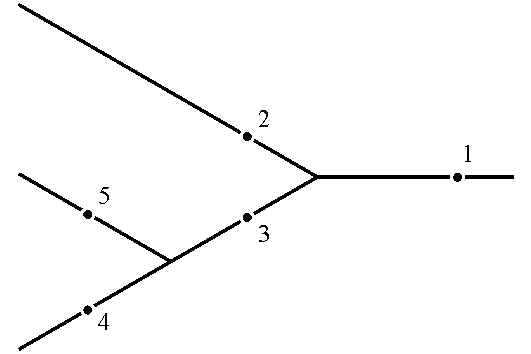
\includegraphics{figures/monitoring_network.pdf}
  \caption{A simple stream monitoring network}
  \label{fig:monitoring_network}
\end{figure}

The connectivity matrix representing this network is
\begin{equation}
  \pmb{C} = \begin{bmatrix}
    1 & -1 & -1 &  0 &  0 \\
    0 &  1 &  0 &  0 &  0 \\
    0 &  0 &  1 & -1 & -1 \\
    0 &  0 &  0 &  1 &  0 \\
    0 &  0 &  0 &  0 &  1
  \end{bmatrix}
\end{equation}
where the flux leaving...
Now show example of the multiplication
\begin{align}
  \pmb{\dot y} &= \pmb{C} \pmb{y} \\
  \begin{bmatrix}
    \dot y_1 \\
    \dot y_2 \\
    \dot y_3 \\
    \dot y_4 \\
    \dot y_5
  \end{bmatrix} &=
                  \begin{bmatrix}
                    y_1 - y_2 - y_3 \\
                    y_2 \\
                    y_3 - y_4 - y_5 \\
                    y_4 \\
                    y_5
                  \end{bmatrix}
\end{align}

A good convention is to construct $\pmb{C}$ as an upper-diagonal matrix.

The inverse of the connectivy matrix forms an accumulation matrix
\begin{equation}
\pmb{y} = \pmb{C}^{-1} \pmb{\dot y}
\end{equation}
where multiplying by $\pmb{C}^{-1}$ is analagous to integration.

A generic load model given by
\begin{equation}
  \pmb{y} = \pmb{C}^{-1} \textit{g}(\pmb{\phi}, \textit{f}(\pmb{\theta}))
\end{equation}
where $\textit{f}()$ and $\textit{g}()$ are functions describing the incremental loadinging and transport efficiency within the network.

In the simplest case
\begin{equation}
  \pmb{\dot y} \sim \pmb{W}x + \mathcal{N}(0, \sigma)
\end{equation}

Similarly,
\begin{equation}
  \pmb{\dot y} \sim \pmb{W}x + \mathcal{N}(0, \sigma)
\end{equation}

Building to neural netowrks or other models

\bibliographystyle{plain}
\bibliography{/home/thodson/org/ref/lib/papers}


\end{document}
